
理解容器和迭代器如何工作的最好方法是,通过创建自己的容器和迭代器来亲身体验。为了避免实现标准库中已经存在的东西,将考虑一些不同的东西——更准确地说,是循环缓冲区。这是一个容器,当它满时,将覆盖现有的元素。可以想象这样一个容器的不同工作方式;因此,首先定义它的需求是很重要的。

\begin{itemize}
\item
容器应该有一个在编译时已知的固定容量,所以不存在运行时内存管理。

\item
容量是容器可以存储的元素数量,大小是容器实际包含的元素数量。当大小等于容量时,容器满了。

\item
容器满时,添加一个新元素将覆盖容器中最旧的元素。

\item
添加新元素总是在最后完成,删除现有元素总是在开头(容器中最旧的元素)完成。

\item
可以通过下标操作符和迭代器对容器的元素进行随机访问。
\end{itemize}

基于这些需求,可以想到以下实现细节:

\begin{itemize}
\item
元素可以存储在数组中,这可以是std::array。

\item
需要两个变量(head和tail)来存储容器的第一个和最后一个元素的索引。因为容器的循环性质,开始和结束会随着时间的推移而变化。

\item
第三个变量将存储容器中的元素数量。没有的话,将无法从头和尾索引的值区分容器是空,还是只有一个元素。

\begin{tcolorbox}[breakable,enhanced jigsaw,colback=blue!5!white,colframe=blue!75!black,title={重要的Note}]
这里展示的实现仅用于教学目的,并不是用于生产的解决方案。有经验的读者会发现实现的不同方面可以优化。但这里的目的是学习如何编写容器,而不是如何优化实现。
\end{tcolorbox}

\end{itemize}

下图显示了这样一个循环缓冲区的可视化表示,容量为八个不同状态的元素:

\begin{center}
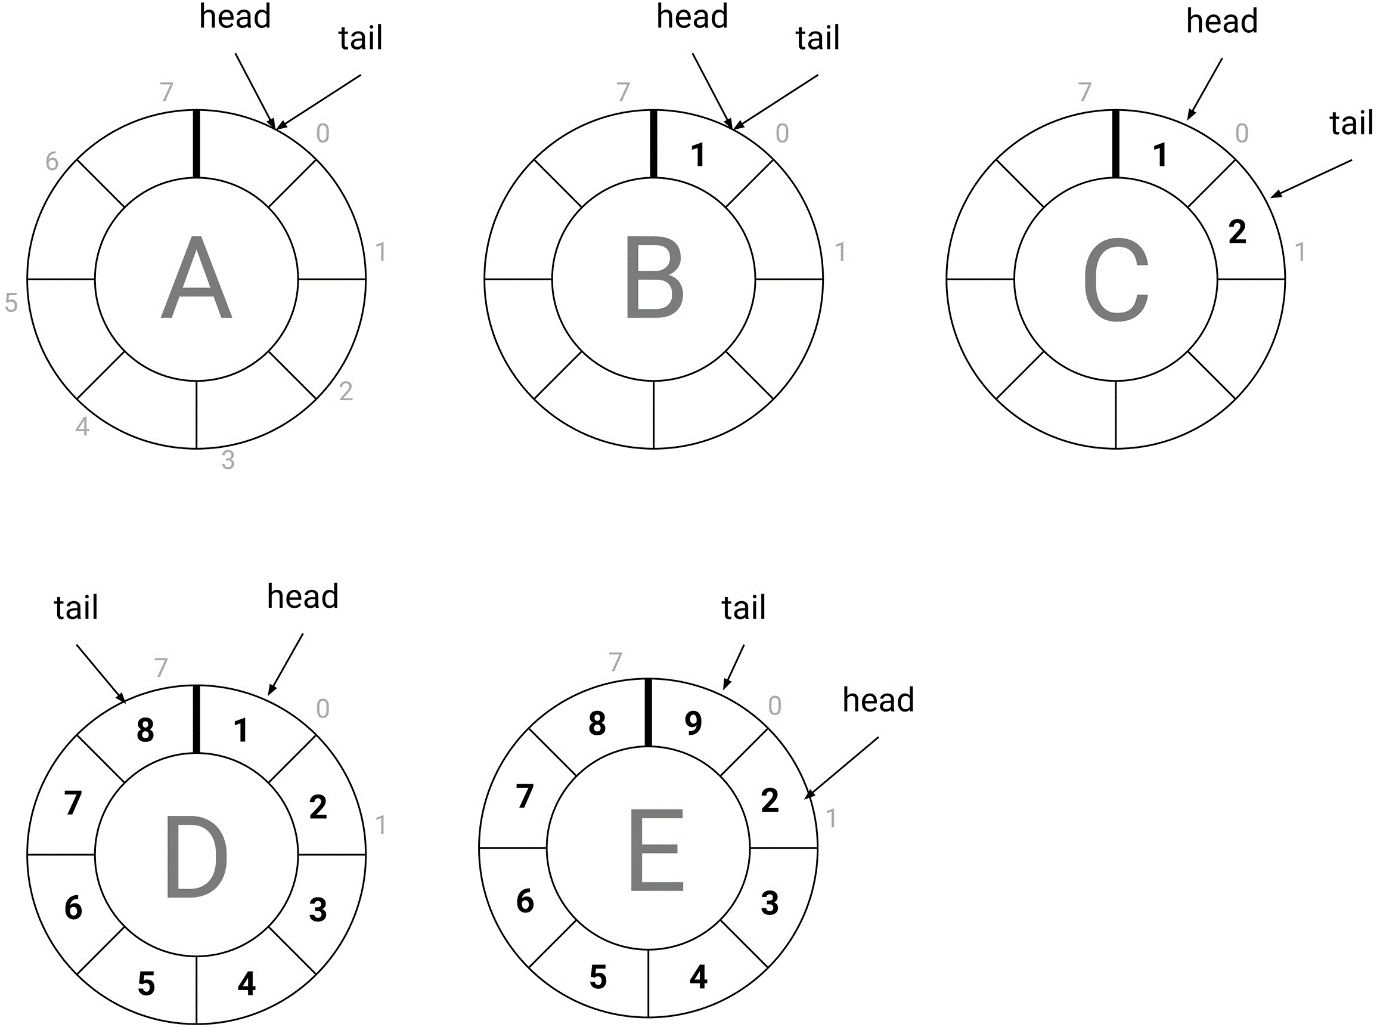
\includegraphics[width=0.8\textwidth]{content/3/chapter8/images/2.png}\\
图 8.2
\end{center}

从这张图中可以看到:

\begin{itemize}
\item
图A:这是一个空缓冲区。容量为8,大小为0,头部和尾部都指向索引0。

\item
图B:缓冲区包含一个元素。容量仍然是8,大小是1,头部和尾部都指向索引0。

\item
图C:缓冲区包含两个元素。大小为2,头部包含索引0,尾部包含索引1。

\item
图D:缓冲区已满。大小为8,等于容量,头部包含索引0,尾部包含索引7。

\item
图E:缓冲区仍然是满的,但是添加了一个额外的元素,触发了缓冲区中最旧元素的覆盖。大小为8,头部包含索引1,尾部包含索引0。
\end{itemize}

现在已经了解了循环缓冲区的语义,可以开始编写实现了,先从容器类开始。

\subsubsubsection{8.2.1\hspace{0.2cm}实现循环缓冲区容器}

容器类的代码太长,所以我们将它分成多个片段。首先是:

\begin{lstlisting}[style=styleCXX]
template <typename T, std::size_t N>
	requires(N > 0)
class circular_buffer_iterator;

template <typename T, std::size_t N>
	requires(N > 0)
class circular_buffer
{
	// ...
};
\end{lstlisting}

这里有两件事:一个是类模板circular\_buffer\_iterator的前向声明,另一个是类模板circular\_buffer。两者都有相同的模板实参,一个类型模板形参T,表示元素的类型,一个非类型模板形参,表示缓冲区的容量。使用约束来确保提供的容量值总是正的。若不支持C++20,可以用static\_assert替换这个约束,或者enable\_if来执行相同的限制。下面的代码段是circular\_buffer类的一部分。

首先,有一系列成员类型定义,为与circular\_buffer类模板相关的不同类型提供别名。这些将在类的实现中使用:

\begin{lstlisting}[style=styleCXX]
	public:
	using value_type = T;
	using size_type = std::size_t;
	using difference_type = std::ptrdiff_t;
	using reference = value_type&;
	using const_reference = value_type const&;
	using pointer = value_type*;
	using const_pointer = value_type const*;
	using iterator = circular_buffer_iterator<T, N>;
	using const_iterator =
	circular_buffer_iterator<T const, N>;
\end{lstlisting}

其次,有存储缓冲区状态的数据成员,元素存储在std::array对象中。head、tail和size都存储在size\_type数据类型的变量中。这些成员都是私有的:

\begin{lstlisting}[style=styleCXX]
private:
	std::array<value_type, N> data_;
	size_type head_ = 0;
	size_type tail_ = 0;
	size_type size_ = 0;
\end{lstlisting}

第三,有实现前面描述的功能的成员函数。以下所有成员都是公开的。首先是构造函数:

\begin{lstlisting}[style=styleCXX]
constexpr circular_buffer() = default;
constexpr circular_buffer(value_type const (&values)[N]) :
	size_(N), tail_(N-1)
{
	std::copy(std::begin(values), std::end(values),
	data_.begin());
}
constexpr circular_buffer(const_reference v):
	size_(N), tail_(N-1)
{
	std::fill(data_.begin(), data_.end(), v);
}
\end{lstlisting}

这里定义了三个构造函数(可以考虑其他的构造函数),初始化空缓冲区的默认构造函数(也是默认构造函数),大小为N的类C数组的构造函数,通过复制数组元素初始化完整缓冲区,最后是接受单个值的构造函数,通过将该值复制到缓冲区的每个元素来初始化完整缓冲区。这些构造函数允许以以下方式创建循环缓冲区:

\begin{lstlisting}[style=styleCXX]
circular_buffer<int, 1> b1; // {}
circular_buffer<int, 3> b2({ 1, 2, 3 }); // {1, 2, 3}
circular_buffer<int, 3> b3(42); // {42, 42, 42}
\end{lstlisting}

接下来,定义了几个成员函数来描述循环缓冲区状态:

\begin{lstlisting}[style=styleCXX]
constexpr size_type size() const noexcept
{ return size_; }

constexpr size_type capacity() const noexcept
{ return N; }

constexpr bool empty() const noexcept
{ return size_ == 0; }

constexpr bool full() const noexcept
{ return size_ == N; }

constexpr void clear() noexcept
{ size_ = 0; head_ = 0; tail_ = 0; };
\end{lstlisting}

size函数返回缓冲区中的元素数量,capacity函数返回缓冲区中可以容纳的元素数量,empty函数检查缓冲区中是否没有元素(与size() == 0相同),full函数检查缓冲区是否已满(与size() == N相同)。还有一个名为clear的函数将循环缓冲区置于空状态,此函数不销毁任何元素(不释放内存或调用析构函数),而只是重置定义缓冲区状态的值。

需要访问缓冲区中的元素,为此定义了以下函数:

\begin{lstlisting}[style=styleCXX]
constexpr reference operator[](size_type const pos)
{
	return data_[(head_ + pos) % N];
}

constexpr const_reference operator[](size_type const pos) const
{
	return data_[(head_ + pos) % N];
}

constexpr reference at(size_type const pos)
{
	if (pos < size_)
		return data_[(head_ + pos) % N];
		
	throw std::out_of_range("Index is out of range");
}

constexpr const_reference at(size_type const pos) const
{
	if (pos < size_)
		return data_[(head_ + pos) % N];
		
	throw std::out_of_range("Index is out of range");
}

constexpr reference front()
{
	if (size_ > 0) return data_[head_];
	throw std::logic_error("Buffer is empty");
}

constexpr const_reference front() const
{
	if (size_ > 0) return data_[head_];
	throw std::logic_error("Buffer is empty");
}

constexpr reference back()
{
	if (size_ > 0) return data_[tail_];
	throw std::logic_error("Buffer is empty");
}

constexpr const_reference back() const
{
	if (size_ > 0) return data_[tail_];
	throw std::logic_error("Buffer is empty");
}
\end{lstlisting}

每个成员都有一个const重载,用于缓冲区的常量实例。常量成员返回一个常量引用,非const成员返回一个正常的引用:

\begin{itemize}
\item
{}[]操作符,返回由其索引指定的元素的引用,而不检查索引的值

\item
at方法的工作原理与下标操作符类似,但检查索引是否小于大小,若小于则抛出异常

\item
front方法,返回对第一个元素的引用;若缓冲区为空,则抛出异常

\item
back方法,返回对最后一个元素的引用;若缓冲区为空,则抛出异常
\end{itemize}

可以使用成员函数来访问元素,也需要成员来向缓冲区中添加和删除元素。添加新元素总是发生在最后,因此称为push\_back。删除现有元素总是发生在最开始(最旧的元素),因此称为pop\_front。让我们先来看看前者:

\begin{lstlisting}[style=styleCXX]
constexpr void push_back(T const& value)
{
	if (empty())
	{
		data_[tail_] = value;
		size_++;
	}
	else if (!full())
	{
		data_[++tail_] = value;
		size_++;
	}
	else
	{
		head_ = (head_ + 1) % N;
		tail_ = (tail_ + 1) % N;
		data_[tail_] = value;
	}
}
\end{lstlisting}

这基于已定义的需求和图8.2中的可视化表示:

\begin{itemize}
\item
若缓冲区为空,则将该值复制到tail\_索引所指向的元素,并增加其大小。

\item
若缓冲区既不空也不满,执行同样的操作,也增加了tail\_索引的值。

\item
若缓冲区已满,则同时增加head\_和tail\_,然后将值复制到tail\_索引所指向的元素。
\end{itemize}

该函数将值参数复制到缓冲区元素,也可以针对推送到缓冲区后不再需要的临时对象或对象进行优化。因此,提供了接受右值引用的重载。这会将值移动到缓冲区,避免不必要的复制。这个重载显示在下面的代码中:

\begin{lstlisting}[style=styleCXX]
constexpr void push_back(T&& value)
{
	if (empty())
	{
		data_[tail_] = value;
		size_++;
	}
	else if (!full())
	{
		data_[++tail_] = std::move(value);
		size_++;
	}
	else
	{
	head_ = (head_ + 1) % N;
	tail_ = (tail_ + 1) % N;
	data_[tail_] = std::move(value);
	}
}
\end{lstlisting}

类似的方法用于实现pop\_back函数来从缓冲区中删除元素:

\begin{lstlisting}[style=styleCXX]
constexpr T pop_front()
{
	if (empty()) throw std::logic_error("Buffer is empty");
	
	size_type index = head_;
	
	head_ = (head_ + 1) % N;
	size_--;
	
	return data_[index];
}
\end{lstlisting}

若缓冲区为空,此函数将抛出异常。否则,将head\_索引的值加1,并返回head\_之前位置的元素的值。下图直观地描述了这一点:

\begin{center}
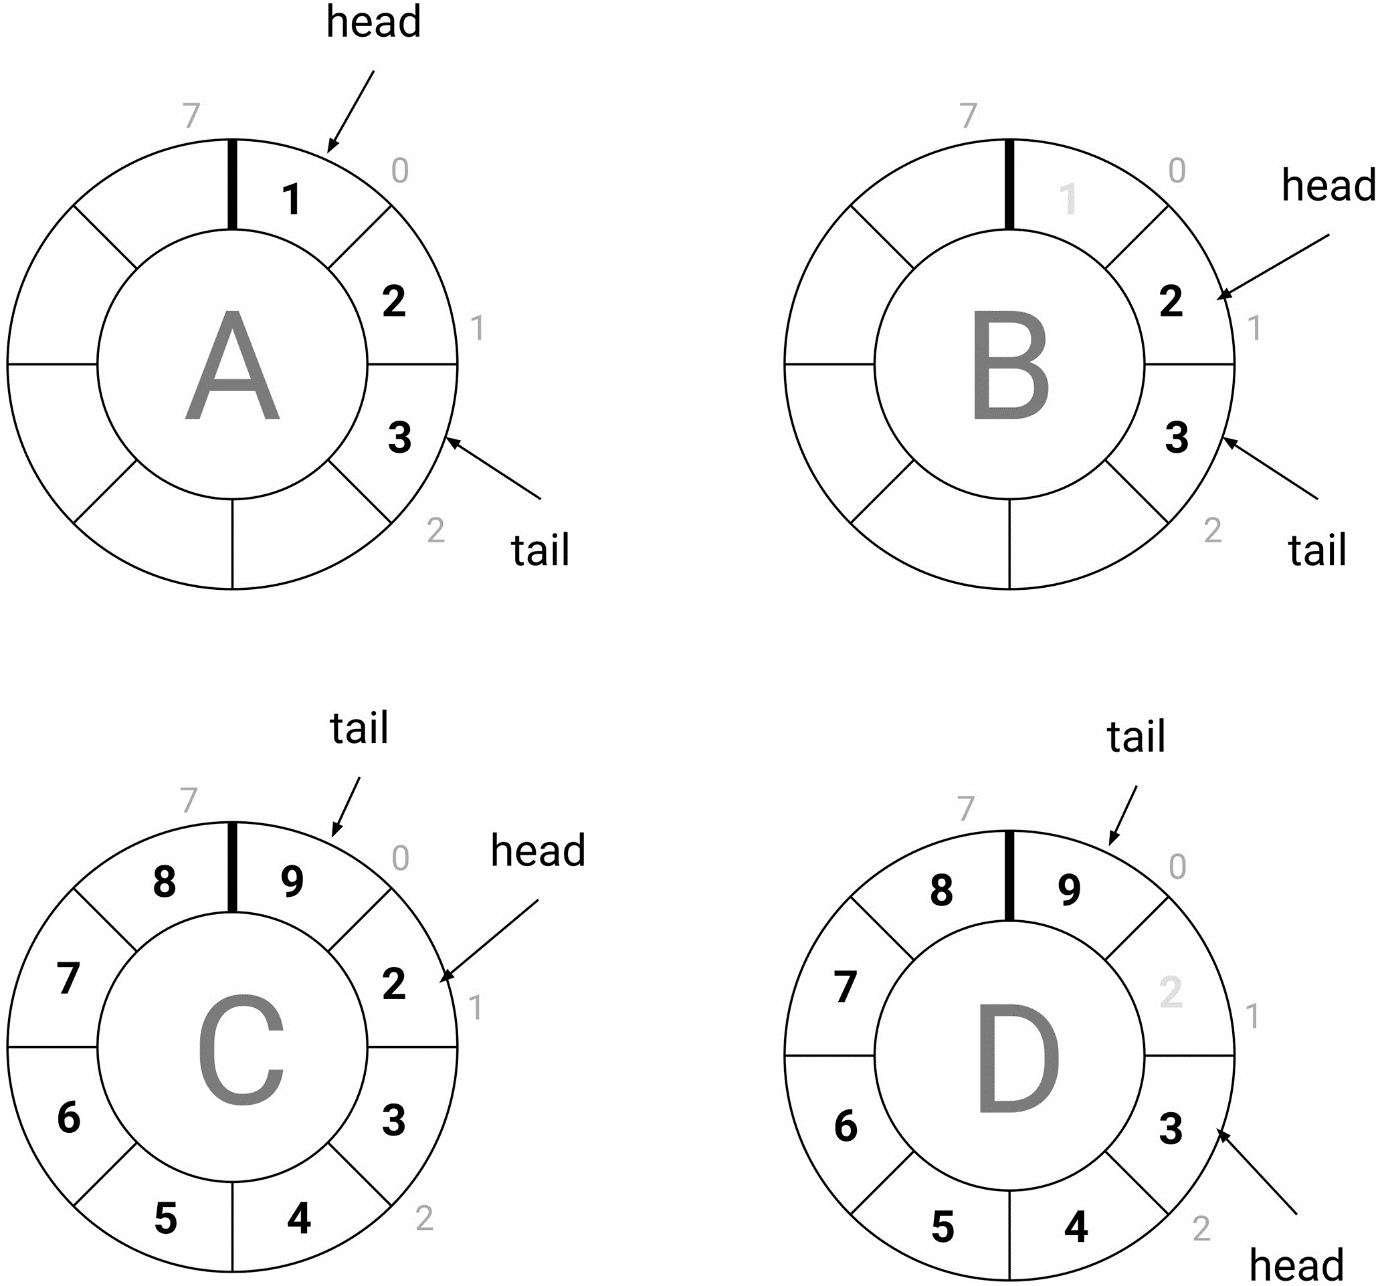
\includegraphics[width=0.7\textwidth]{content/3/chapter8/images/3.png}\\
图 8.3
\end{center}

可以看到:

\begin{itemize}
\item
图A:缓冲区有3个元素(1、2和3),头在索引0,尾在索引2。

\item
图B:前面删除了一个索引为0的元素。头部现在是指数1,尾部仍然是指数2。缓冲区现在有两个元素。

\item
图C:缓冲区有8个元素,这是其最大容量,一个元素已经覆盖。头部在索引1,尾部在索引0。

\item
图D:前面删除了一个元素,即索引1。头部现在在索引2,尾部仍然在索引0。缓冲区现在有7个元素。
\end{itemize}

下面的代码展示了同时使用push\_back和pop\_front的例子:

\begin{lstlisting}[style=styleCXX]
circular_buffer<int, 4> b({ 1, 2, 3, 4 });
assert(b.size() == 4);

b.push_back(5);
b.push_back(6);
b.pop_front();

assert(b.size() == 3);
assert(b[0] == 4);
assert(b[1] == 5);
assert(b[2] == 6);
\end{lstlisting}

最后,成员函数begin和end返回指向缓冲区中第一个和倒数第一个元素的迭代器:

\begin{lstlisting}[style=styleCXX]
iterator begin()
{
	return iterator(*this, 0);
}

iterator end()
{
	return iterator(*this, size_);
}

const_iterator begin() const
{
	return const_iterator(*this, 0);
}

const_iterator end() const
{
	return const_iterator(*this, size_);
}
\end{lstlisting}

为了理解这些,需要了解迭代器类实际上是如何实现的。我们将在下一节中对此进行探讨。

\subsubsubsection{8.2.2\hspace{0.2cm}为循环缓冲区容器实现迭代器类型}

上一节开始使用circular\_buffer容器时声明了迭代器类模板,但也需要定义它的实现。然而,还有一件事必须做:为了使迭代器类能够访问容器的私有成员,需要声明为友元:

\begin{lstlisting}[style=styleCXX]
private:
	friend circular_buffer_iterator<T, N>;
\end{lstlisting}

来看看circular\_buffer\_iterator类,与容器类有相似之处。这包括模板参数、约束和成员类型集(其中一些与circular\_buffer中的成员类型相同):

\begin{lstlisting}[style=styleCXX]
template <typename T, std::size_t N>
requires(N > 0)
class circular_buffer_iterator
{
public:
	using self_type = circular_buffer_iterator<T, N>;
	using value_type = T;
	using reference = value_type&;
	using const_reference = value_type const &;
	using pointer = value_type*;
	using const_pointer = value_type const*;
	using iterator_category =
		std::random_access_iterator_tag;
	using size_type = std::size_t;
	using difference_type = std::ptrdiff_t;
public:
	/* definitions */
	
private:
	std::reference_wrapper<circular_buffer<T, N>> buffer_;
	size_type index_ = 0;
};
\end{lstlisting}

circular\_buffer\_iterator类有一个对循环缓冲区的引用,以及其所指向的缓冲区中元素的索引。circular\_buffer<T, N>的引用包装在std::reference\_wrapper对象中。可以通过提供这两个参数显式地创建这样的迭代器,构造函数如下所示:

\begin{lstlisting}[style=styleCXX]
explicit circular_buffer_iterator(
	circular_buffer<T, N>& buffer,
	size_type const index):
	buffer_(buffer), index_(index)
{ }
\end{lstlisting}

若现在回顾circular\_buffer的begin和end成员函数的定义,可以看到第一个参数是*this,第二个参数是0 (begin迭代器),size\_(end迭代器)。第二个值是迭代器指向的元素头部的偏移量。因此,0是第一个元素,而size\_是缓冲区中最后一个元素。

这里,需要随机访问缓冲区的元素,所以迭代器类别是随机迭代器。成员类型iterator\_category是std::random\_access\_iterator\_tag的别名。因此,需要提供这样一个迭代器所支持的所有操作。本章的前一节中,讨论了迭代器类别,以及每个类别所需的操作。接下来我们将逐一进行实现。

从输入迭代器开始:

\begin{lstlisting}[style=styleCXX]
self_type& operator++()
{
	if(index_ >= buffer_.get().size())
		throw std::out_of_range("Iterator cannot be
								incremented past the end of the range");
								
	index_++;
	return *this;
}

self_type operator++(int)
{
	self_type temp = *this;
	++*this;
	return temp;
}

bool operator==(self_type const& other) const
{
	return compatible(other) && index_ == other.index_;
}

bool operator!=(self_type const& other) const
{
	return !(*this == other);
}

const_reference operator*() const
{
	if (buffer_.get().empty() || !in_bounds())
		throw std::logic_error("Cannot dereferentiate the
	iterator");
	return buffer_.get().data_[
		(buffer_.get().head_ + index_) %
		 buffer_.get().capacity()];
}

const_reference operator->() const
{
	if (buffer_.get().empty() || !in_bounds())
		throw std::logic_error("Cannot dereferentiate the
								iterator");
								
	return buffer_.get().data_[
		(buffer_.get().head_ + index_) %
		 buffer_.get().capacity()];
}
\end{lstlisting}

这里实现了递增(前缀和后缀)、检查相等/不相等,以及解引用。*和->操作符在无法解引用元素时抛出异常。这种情况发生在缓冲区为空时,或者索引不在边界内(在head\_和tail\_之间)。使用了两个辅助函数(都是私有的),分别称为compatible和is\_bounds:

\begin{lstlisting}[style=styleCXX]
bool compatible(self_type const& other) const
{
	return buffer_.get().data_.data() ==
		   other.buffer_.get().data_.data();
}

bool in_bounds() const
{
	return
		!buffer_.get().empty() &&
		(buffer_.get().head_ + index_) %
		 buffer_.get().capacity() <= buffer_.get().tail_;
}
\end{lstlisting}

前向迭代器是输入迭代器,同时也是输出迭代器。之前看到的那些用于输入迭代器的迭代器,因为对可解引用的前向迭代器执行操作会使其迭代器值解引用,所以前向迭代器可以用于多遍算法。若a和b是两个前向迭代器并且相等,要么不可解引用;否则,其迭代器值*a和*b指向同一个对象。反之亦然,若*a和*b相等,那么a和b也相等。这对于我们的实现来说是正确的。

前向迭代器的另一个要求是是可交换的。若a和b是两个前向迭代器,那么swap(a, b)应该是一个有效的操作。回到使用std::reference\_wrapper对象来保存对循环\_buffer<T, N>的引用。引用是不可交换的,所以circular\_buffer\_iterator不可交换。然而,std::reference\_wrapper可交换,这也使得我们的迭代器类型可交换。可以使用static\_assert进行验证:

\begin{lstlisting}[style=styleCXX]
static_assert(
	std::is_swappable_v<circular_buffer_iterator<int, 10>>);
\end{lstlisting}

\begin{tcolorbox}[breakable,enhanced jigsaw,colback=blue!5!white,colframe=blue!75!black,title={重要的Note}]
std::reference\_wrapper的另一种替代方法是使用指向circular\_buffer类的原始指针,因为指针可以赋值,因此是可交换的。使用哪一种就看开发者的开发风格和个人喜好。本例中,我倾向于避免使用原始指针的解决方案。
\end{tcolorbox}

为了满足双向迭代器类别的要求,需要支持递减。下一个代码段中,可以看到前缀和后缀递减操作符的实现:

\begin{lstlisting}[style=styleCXX]
self_type& operator--()
{
	if(index_ <= 0)
		throw std::out_of_range("Iterator cannot be
			decremented before the beginning of the range");
			
	index_--;
	return *this;
}

self_type operator--(int)
{
	self_type temp = *this;
	--*this;
	return temp;
}
\end{lstlisting}

最后,因为需要实现随机迭代器。首先要实现的需求是算术(+和-)和复合(+=和-=)操作:

\begin{lstlisting}[style=styleCXX]
self_type operator+(difference_type offset) const
{
	self_type temp = *this;
	return temp += offset;
}

self_type operator-(difference_type offset) const
{
	self_type temp = *this;
	return temp -= offset;
}

difference_type operator-(self_type const& other) const
{
	return index_ - other.index_;
}

self_type& operator +=(difference_type const offset)
{
	difference_type next =
		(index_ + next) % buffer_.get().capacity();
	if (next >= buffer_.get().size())
		throw std::out_of_range("Iterator cannot be
								 incremented past the bounds of the range");
								 
	index_ = next;
	return *this;
}

self_type& operator -=(difference_type const offset)
{
	return *this += -offset;
}
\end{lstlisting}

随机访问迭代器必须支持与其他操作的不相等比较,需要重载<、<=、>和>=操作符,但<=、>和>=操作符可以基于<操作符实现。其定义如下所示:

\begin{lstlisting}[style=styleCXX]
bool operator<(self_type const& other) const
{
	return index_ < other.index_;
}

bool operator>(self_type const& other) const
{
	return other < *this;
}

bool operator<=(self_type const& other) const
{
	return !(other < *this);
}

bool operator>=(self_type const& other) const
{
	return !(*this < other);
}
\end{lstlisting}

最后,但同样重要的是,需要使用下标操作符([])提供对元素的访问。可能的实现如下所示:

\begin{lstlisting}[style=styleCXX]
value_type& operator[](difference_type const offset)
{
	return *((*this + offset));
}

value_type const & operator[](difference_type const offset)
const
{
	return *((*this + offset));
}
\end{lstlisting}

至此,我们已经完成了循环缓冲区迭代器类型的实现。若在理解这两个类的大量代码片段时遇到困难,可以在本书的GitHub存储库中找到完整实现。下面是使用迭代器类型的简单示例:

\begin{lstlisting}[style=styleCXX]
circular_buffer<int, 3> b({1, 2, 3});
std::vector<int> v;
for (auto it = b.begin(); it != b.end(); ++it)
{
	v.push_back(*it);
}
\end{lstlisting}

这段代码实际上可以通过基于范围的for循环来简化。这里,我们不直接使用迭代器,但编译器生成的代码可以。因此,下面的代码段相当于前面的代码段:

\begin{lstlisting}[style=styleCXX]
circular_buffer<int, 3> b({ 1, 2, 3 });
std::vector<int> v;
for (auto const e : b)
{
	v.push_back(e);
}
\end{lstlisting}

但这里为circular\_buffer\_iterator提供的实现,不能使以下代码段编译通过:

\begin{lstlisting}[style=styleCXX]
circular_buffer<int, 3> b({ 1,2,3 });
*b.begin() = 0;

assert(b.front() == 0);
\end{lstlisting}

这要求我们能够通过迭代器写入元素,但我们的实现不满足输出迭代器类别的要求。这要求表达式如*it = v,或*it++ = v是有效的。为此,需要提供返回非const引用类型的*和->操作符的非const重载方式:

\begin{lstlisting}[style=styleCXX]
reference operator*()
{
	if (buffer_.get().empty() || !in_bounds())
		throw std::logic_error("Cannot dereferentiate the
								iterator");
	
	return buffer_.get().data_[
		(buffer_.get().head_ + index_) %
		 buffer_.get().capacity()];
}

reference operator->()
{
	if (buffer_.get().empty() || !in_bounds())
		throw std::logic_error("Cannot dereferentiate the
								iterator");
								
	return buffer_.get().data_[
		(buffer_.get().head_ + index_) %
		 buffer_.get().capacity()];
}
\end{lstlisting}

GitHub库中可以找到更多带迭代器和不带迭代器的circular\_buffer类的示例。接下来,我们将把注意力集中在实现一个适用于任何范围的通用算法上,包括在这里定义的circular\_buffer容器。






















